\documentclass{article}

\usepackage[preprint]{neurips_2025}
\usepackage{graphicx}
\usepackage{booktabs}
\usepackage{amsmath}
\usepackage{caption}
\usepackage[hidelinks]{hyperref}
\captionsetup{font=small,skip=3pt}
\setlength{\textfloatsep}{8pt plus 2pt minus 2pt}
\setlength{\floatsep}{8pt plus 2pt minus 2pt}
\setlength{\intextsep}{8pt plus 2pt minus 2pt}
\setlength{\abovecaptionskip}{3pt}
\setlength{\belowcaptionskip}{0pt}

\title{Generating Chest X-rays with a Variational Autoencoder}

\author{Lukelaitw \\ ECE 285, University of California San Diego}

\begin{document}
\maketitle

\begin{abstract}
We train a convolutional variational autoencoder on the Kaggle chest X-ray collection and draw new $64\times 64$ radiographs from the prior.
Held-out reconstruction and KL curves, plus pytorch-ignite Inception Score and FID, show recognizable but blurry samples.
ImageNet-based scores are only a coarse check.
Code is available at \url{https://github.com/Lukelaitw/2026Fall-UCSD-ECE285-HW1}.
\end{abstract}

\section{Method}
The encoder uses four stride-2 convolutions, $1\!\to\!32\!\to\!64\!\to\!128\!\to\!256$, with kernel size 4, padding 1, and LeakyReLU$(0.2)$.
The $256\times 4\times 4$ map is flattened to $\mu$ and $\log\sigma^2$.
A code is $z=\mu+\exp(\tfrac12\log\sigma^2)\,\epsilon$, $\epsilon\sim\mathcal{N}(0,I)$.
The decoder expands $z$ to $256\times 4\times 4$ and applies transposed convolutions $256\!\to\!128\!\to\!64\!\to\!32\!\to\!1$, with ReLU activations and a final sigmoid.
There is no batch normalization.
The model has 2,955,201 parameters.
After training, samples are $\mathrm{decode}(z)$ for $z$ drawn from the standard normal; the encoder is not used.

Both loss terms are summed over one image and then averaged over the batch of $B$ images,
\begin{equation}
\mathcal{L}
= \frac{1}{B}\sum_{i}\mathrm{BCE}(\hat x_i, x_i)
- \frac{1}{2B}\sum_{i,j}\bigl(1+\log\sigma^2_{ij}-\mu_{ij}^2-e^{\log\sigma^2_{ij}}\bigr).
\end{equation}
The KL weight is 1.
Summing the pixel BCE, rather than averaging over the 4,096 pixels, keeps reconstruction on the same scale as the KL term.

\section{Setup}
Films are converted to grayscale, bilinearly resized to $64\times 64$, and scaled to $[0,1]$.
Aspect ratios from about $0.84$ to $3.38$ are stretched to a square.
We do not flip images, because the heart would change sides, and we do not map pixels to $[-1,1]$, because the decoder ends in a sigmoid.
Labels are unused.
Training uses 5,216 images and test loss uses 624; the 16-image validation split is ignored.
Table~\ref{tab:hparams} lists the optimizer settings.
Seed 42 fixes initialization, minibatch order, the sample sheet, and the evaluation indices.

\begin{table}[ht]
\centering
\caption{Training hyperparameters.}
\label{tab:hparams}
\small
\begin{tabular}{lc}
\toprule
Setting & Value \\
\midrule
Image & $64\times 64$ grayscale \\
Latent dimension & 128 \\
Optimizer & Adam, learning rate $10^{-3}$ \\
Batch size / epochs & 128 / 1000 \\
KL weight / seed & 1 / 42 \\
\bottomrule
\end{tabular}
\end{table}

\section{Results}
Figure~\ref{fig:loss} separates total loss, reconstruction, and KL.
Most of the drop is in the first 20 epochs.
At epoch 1000, training loss is 2376.3 (reconstruction 2353.0, KL 23.3) and test loss is 2393.3 (reconstruction 2370.5, KL 22.9).
The test curve stays close to training, so the blur is not explained by overfitting.
KL rises from about 8 to about 23 and then holds, so the latent codes do not collapse to the prior.

\begin{figure}[ht]
\centering
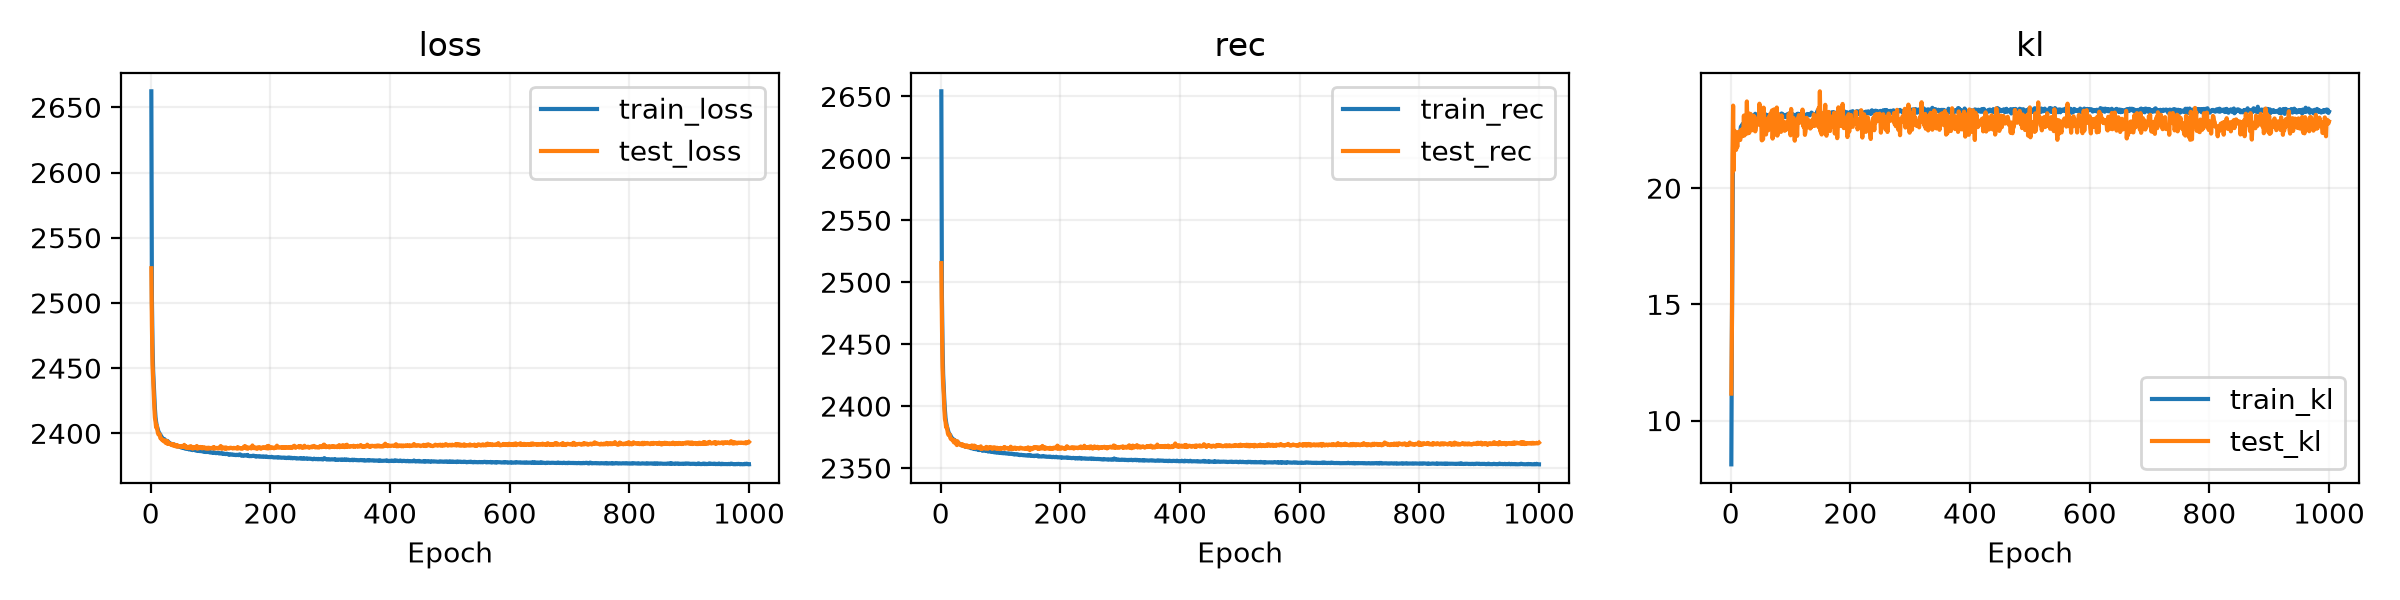
\includegraphics[width=\linewidth]{figures/loss.png}
\caption{Train and test curves. KL is plotted alone because it is much smaller than reconstruction.}
\label{fig:loss}
\end{figure}

IS and FID use pytorch-ignite 0.5.5 and the default ImageNet Inception-v3 1000-class probabilities, not 2048-dimensional features.
Grayscale inputs are bilinearly resized to $299\times 299$, repeated to three channels, and kept in $[0,1]$.
FID compares 2,000 prior samples with the first 2,000 images of a seed-42 permutation of the training split; IS uses only the samples.
A disjoint block of 2,000 real images is the matched control.
The scored checkpoint is \texttt{epoch\_1000.pt} on MPS (PyTorch 2.11.0, torchvision 0.26.0).
Course-guide rows in Table~\ref{tab:scores} share this resolution, count, and probability FID, but not this split.

\begin{table}[ht]
\centering
\caption{IS and FID with 2,000 images per set. Lower FID and higher IS are better.}
\label{tab:scores}
\small
\begin{tabular}{lcc}
\toprule
Comparison & FID$\downarrow$ & IS$\uparrow$ \\
\midrule
Real vs.\ real (this code) & 0.0011 & 2.206 \\
VAE samples vs.\ real & 0.078 & 1.883 \\
Course guide, real vs.\ real & 0.0006 & 2.19 \\
Course guide, repeated mean image & 0.21 & 1.00 \\
Course guide, heavily blurred real & 0.24 & 1.20 \\
\bottomrule
\end{tabular}
\end{table}

The VAE FID of 0.078 is above the real baseline and below the guide's constant-image and blurred-film failures.
SciPy reported an ill-conditioned covariance, so that FID is approximate, and the IS of 1.88 lies between those failures and real films.
Figure~\ref{fig:images} is a frozen 64-sample sheet plus 32 test reconstructions; the table uses 2,000 independent draws.

\begin{figure}[ht]
\centering
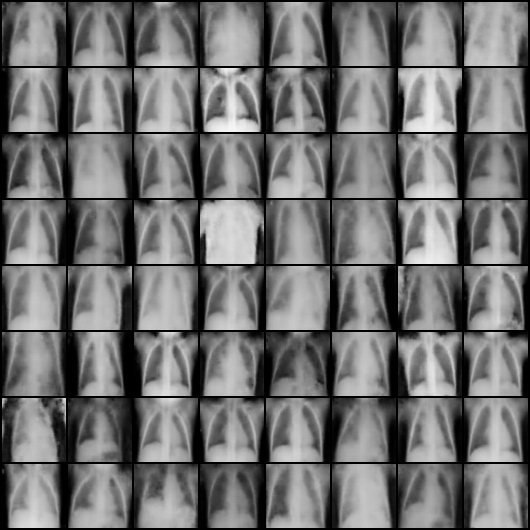
\includegraphics[height=1.28in]{figures/samples.png}\hfill
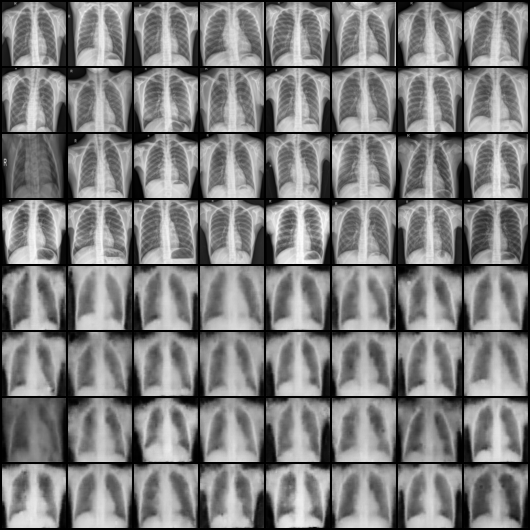
\includegraphics[height=1.28in]{figures/reconstructions.png}
\caption{Left: 64 samples from the epoch-1000 decoder. Right: 32 test images (top) and reconstructions (bottom).}
\label{fig:images}
\end{figure}

\section{Discussion}
Samples show a chest, ribs, and a mediastinum, and lung width and brightness vary, so this is not a collapsed prior.
They are blurry because pixelwise BCE predicts the mean anatomy for each $z$ while the KL term pulls codes toward $\mathcal{N}(0,I)$.
Reconstructions keep layout but lose focal opacities, side markers, and fine ribs.
A lower KL weight, a wider latent code, $128\times 128$ images, or a perceptual loss are the next levers.
IS and FID are weak on this data: ImageNet has no X-rays, real films score only about 2.2, and this probability FID is not the usual 2048-dimensional score.

\end{document}
